In this appendix, I provide details on the methodology for the simulations and decompositions in section \ref{chap1-counterfactual}. The benchmark simulation is the one obtained in section \ref{chap1-model_pred}. In what follows, a variable with a prime denotes the new value of this variable that is used in the counterfactual simulation. 

\textbf{Factor-accumulation counterfactual simulation.} I neutralize the factor accumulation effect by setting the rate of population growth and the survival rate at their levels in 1970, i.e. $n^\prime_t = n_{1970}$ and $p^\prime_t = p_{1970}$.
The expected survival rate $p_{t+1}$ of one generation is the survival rate $p_t$ once this generation becomes old, therefore it implies that $p_{t+1}^\prime = p_t^\prime = p_{1970}$.
Thus, the numbers of young and old households in the first period of each sequence, i.e. from 1970 to 2000, are recalculated to be consistent, such that
\begin{equation*}
    N_t^{y\prime} = \frac{n^\prime_t}{n_t} \times N_t^y  ~\text{ and }~    N_t^{o\prime} = \frac{p^\prime_t}{p_t} \times N_t^o,
\end{equation*}
This change affects demographic dynamics, which are therefore recalculated for the second and third periods of each sequence, i.e. from 2010 to 2080, such that
\begin{equation*}
    N_t^{y\prime} = n^\prime_t N_{t-1}^{y\prime} ~\text{ and }~    N_t^{o\prime} = p_t N_{t-1}^{y\prime}.
\end{equation*}
The capital stock in the first period of each sequence, i.e. from 1970 to 2000, is recalculated such that
\begin{equation*}
    K_t^\prime = \frac{1+\alpha p_t}{\alpha p_t}\frac{\alpha p_t^\prime}{1+\alpha p_t^\prime} K_t.
\end{equation*}
The initial capital stocks are recalculated because setting constant the survival rate implies changes in the saving rate as
\begin{equation*}
    K_t \equiv S_{t-1} = \frac{\alpha p_t}{1+\alpha p_t} Y^y_{t-1},
\end{equation*}
where $Y^y_{t-1}$ is the aggregate net income of young households.
Thus, not taking into account the change in the saving rate would bias the interpretation of the effect of survival rate dynamics by leaving behind part of the effect that occurs through capital accumulation.

\textbf{Policy-mechanism counterfactual simulation.} I neutralize the policy-mechanism effect by setting only the political weight of the young at its level in 1970, i.e. $\eta_t^\prime = \eta_{1970}$. All other demographic variables remain identical to the benchmark simulation.

\textbf{Baseline counterfactual simulation.} I neutralize both effects, therefore, I set $n^\prime_t = n_{1970}$, $p^\prime_t = p^\prime_{t+1} = p_{1970}$. This simulation is the combination of the two previous ones. As before, the number of young and old households along with the capital stock at first period of each sequence, i.e. from 1970 to 2000, are recalculated. These changes affect the dynamics of young and old households which are therefore recalculated for the second and third periods of each sequence, i.e. from 2010 to 2080.
For every year, the political weight of the young remains at its level in 1970, i.e. $\eta^\prime_t = \eta_{1970}$

\textbf{Factor accumulation versus policy mechanism.} 

Figure \ref{chap1-fig:quant-counter-channel} presents the labor share from the four counterfactual simulations, as detailed above.
\begin{figure}[!htb]
	\centering
	\caption{Counterfactual simulations of the channels of demographic changes.} \label{chap1-fig:quant-counter-channel}
	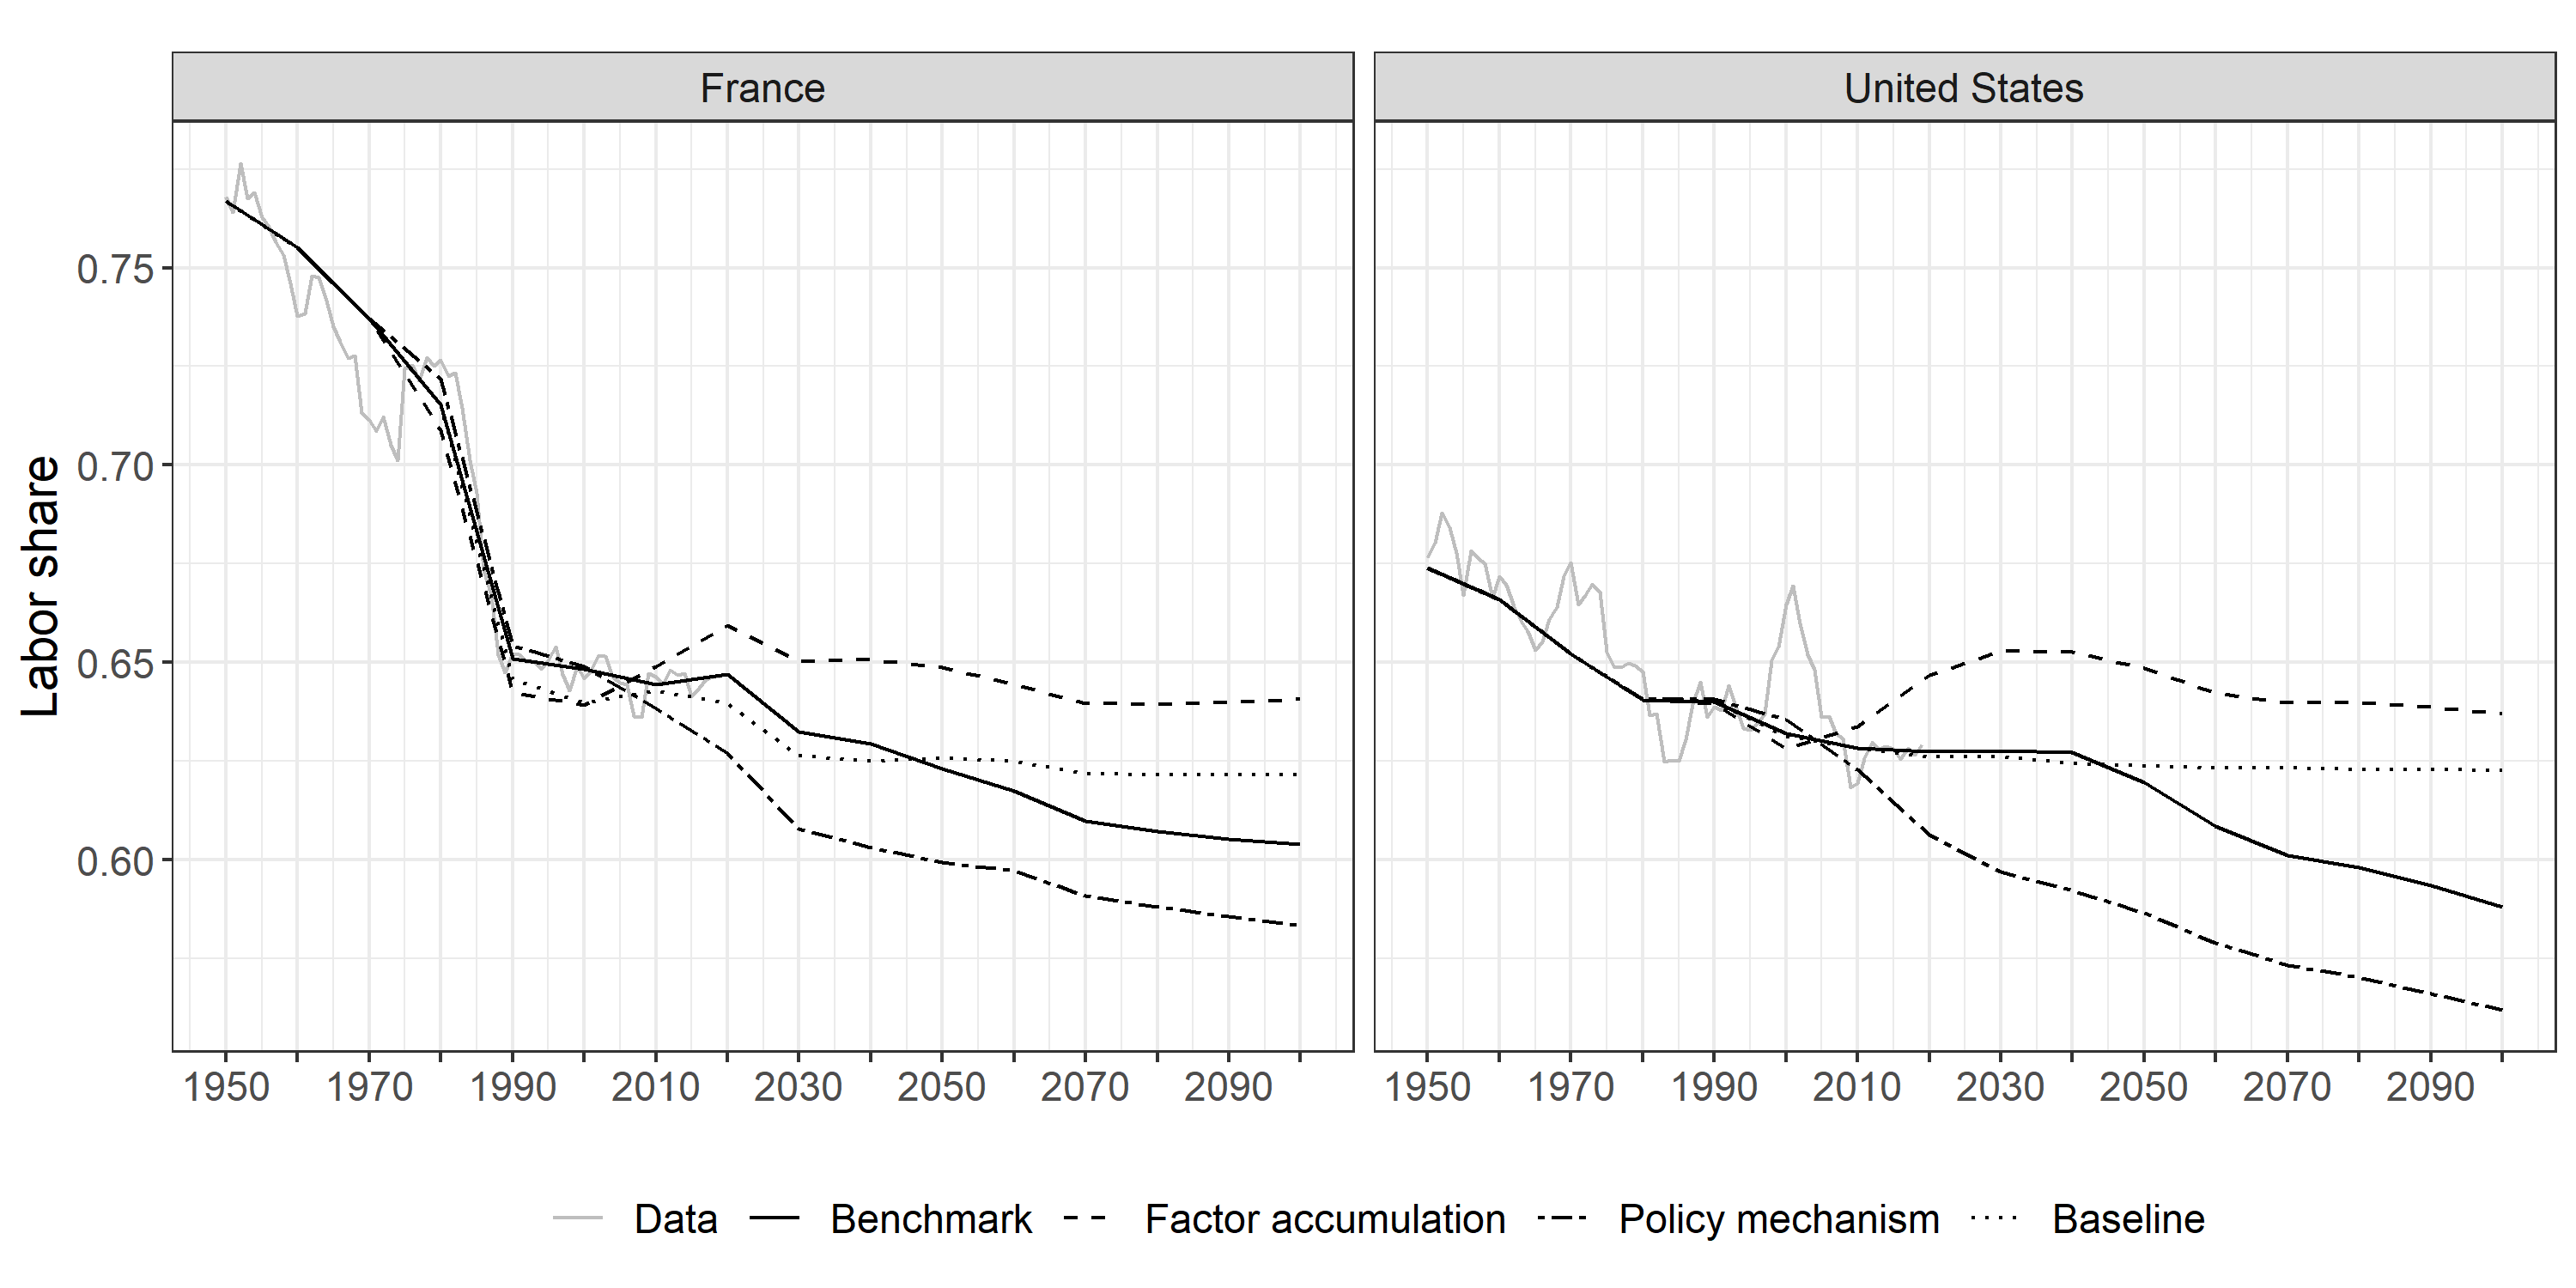
\includegraphics[width=1\linewidth]{chap1/graphic/quant-counter-channel.png}
	\vspace{-3em}
	\justify\singlespacing\footnotesize\textit{Notes:} The figure shows the counterfactual simulations of the channels of demographic changes on the labor share. 
	Labor share data are from the \href{https://www.rug.nl/ggdc/productivity/pwt/}{Penn World Table 9.1} with self-employed income as labor compensation.
	The benchmark labor share corresponds to the benchmark predictions of the model. The factor-accumulation simulation refers to the labor share of the counterfactual simulation in which the factor-accumulation channel is neutralized. The policy-mechanism simulation refers to the labor share of the counterfactual simulation in which the policy-mechanism channel is neutralized. The baseline labor share corresponds to the predictions when both channels are neutralized.
\end{figure}
From this figure, I derive the decomposition of the channels of demographic changes, see figure \ref{chap1-fig:quant-decomp-channel}.